% !TEX TS-program = XeLaTeX
% use the following command: 
% all document files must be coded in UTF-8
\documentclass{textolivre}
% See more information on the repository: https://github.com/leolca/textolivre

% Metadata
\begin{filecontents*}[overwrite]{article.xmpdata}
    \Title{Transletramentos: o ensino de Língua Portuguesa mediado pelas TDIC}
    \Author{Adriane Elisa Glasser \sep Maria Elena Pires Santos}
    \Language{pt-BR}
    \Keywords{Linguística Aplicada \sep transletramentos \sep saberes locais \sep tecnologias digitais de informação e comunicação}
    \Journaltitle{Texto Livre}
    \Journalnumber{1983-3652}
    \Volume{14}
    \Issue{3}
    \Firstpage{1}
    \Lastpage{17}
    \Doi{10.35699/1983-3652.2021.29627}

    \setRGBcolorprofile{sRGB_IEC61966-2-1_black_scaled.icc}
            {sRGB_IEC61966-2-1_black_scaled}
            {sRGB IEC61966 v2.1 with black scaling}
            {http://www.color.org}
\end{filecontents*}

\journalname{Texto Livre}
\thevolume{14}
\thenumber{3}
\theyear{2021}
\receiveddate{\DTMdisplaydate{2021}{2}{24}{-1}} % YYYY MM DD
\accepteddate{\DTMdisplaydate{2021}{4}{14}{-1}}
\publisheddate{\DTMdisplaydate{2021}{8}{4}{-1}}
% Corresponding author
\corrauthor{Adriane Elisa Glasser}
% DOI
\articledoi{10.35699/1983-3652.2021.29627}
%\articleid{NNNN} % if the article ID is not the last 5 numbers of its DOI, provide it using \articleid{} commmand
% list of available sesscions in the journal: articles, dossier, reports, essays, reviews, interviews, editorial
\articlesessionname{articles}
% Abbreviated author list for the running footer
\runningauthor{Glasser e Santos}
\sectioneditorname{Bárbara Amaral da Silva}
\layouteditorname{Leonado Araújo}

\title{Transletramentos: o ensino de língua portuguesa mediado pelas TDIC}
\othertitle{Transliteracy: Portuguese language teaching mediated by ICDT}
% if there is a third language title, add here:
%\othertitle{Artikelvorlage zur Einreichung beim Texto Livre Journal}

\author[1]{Adriane Elisa Glasser \orcid{0000-0003-4348-4386} \thanks{Email: \url{adriane.glasser@gmail.com}}}
\author[2]{Maria Elena Pires Santos \orcid{0000-0002-1979-2090} \thanks{Email: \url{mel.pires@hotmail.com}}}

\affil[1]{Universidade Estadual do Oeste do Paraná, Faculdade de Letras, Centro de Educação, Letras e Saúde - Foz do Iguaçu, PR, Brasil.}
\affil[2]{Universidade Estadual do Oeste do Paraná, Programa de pós-graduação Mestrado/Doutorado em Letras, Cascavel, PR, Brasil.}


\addbibresource{article.bib}
% use biber instead of bibtex
% $ biber tl-article-template

% set language of the article
%\setdefaultlanguage{french}
\setdefaultlanguage{portuguese}
\setotherlanguage{english}

% for spanish, use:
%\setdefaultlanguage{spanish}
%\gappto\captionsspanish{\renewcommand{\tablename}{Tabla}} % use 'Tabla' instead of 'Cuadro'
%\AfterEndPreamble{\crefname{table}{tabla}{tablas}\Crefname{table}{Tabla}{Tablas}}

% for languages that use special fonts, you must provide the typeface that will be used
% \setotherlanguage{arabic}
% \newfontfamily\arabicfont[Script=Arabic]{Amiri}
% \newfontfamily\arabicfontsf[Script=Arabic]{Amiri}
% \newfontfamily\arabicfonttt[Script=Arabic]{Amiri}
%
% in the article, to add arabic text use: \textlang{arabic}{ ... }

% to use emoticons in your manuscript
% https://stackoverflow.com/questions/190145/how-to-insert-emoticons-in-latex/57076064
% using font Symbola, which has full support
% the font may be downloaded at:
% https://dn-works.com/ufas/
% add to preamble:
% \newfontfamily\Symbola{Symbola}
% in the text use:
% {\Symbola }

% reference itens in a descriptive list using their labels instead of numbers
% insert the code below in the preambule:
\makeatletter
\let\orgdescriptionlabel\descriptionlabel
\renewcommand*{\descriptionlabel}[1]{%
  \let\orglabel\label
  \let\label\@gobble
  \phantomsection
  \edef\@currentlabel{#1\unskip}%
  \let\label\orglabel
  \orgdescriptionlabel{#1}%
}
\makeatother
%
% in your document, use as illustraded here:
%\begin{description}
%  \item[first\label{itm1}] this is only an example;
%  % ...  add more items
%\end{description}
 

% custom epigraph - BEGIN 
%%% https://tex.stackexchange.com/questions/193178/specific-epigraph-style
\usepackage{epigraph}
\renewcommand\textflush{flushright}
\makeatletter
\newlength\epitextskip
\pretocmd{\@epitext}{\em}{}{}
\apptocmd{\@epitext}{\em}{}{}
\patchcmd{\epigraph}{\@epitext{#1}\\}{\@epitext{#1}\\[\epitextskip]}{}{}
\makeatother
\setlength\epigraphrule{0pt}
\setlength\epitextskip{0.5ex}
\setlength\epigraphwidth{.7\textwidth}
% custom epigraph - END


% if you use multirows in a table, include the multirow package
\usepackage{multirow}

% add line numbers for submission
%\usepackage{lineno}
%\linenumbers


\begin{document}
\maketitle

\begin{polyabstract}
\begin{abstract}
A ampliação das Tecnologias Digitais de Informação e Comunicação (TDIC) no contexto escolar abre espaço para que a centralidade do ensino - que, quase sempre, recai sobre a figura do professor e/ou do aluno - se estabeleça na ‘aprendência’ enquanto processo \cite{assmann2001}. Desse modo, situadas na área da Linguística Aplicada \cite{kleiman2007} e à luz da pesquisa qualitativa/interpretativista e etnográfica \cite{denzin2006}, objetivamos discutir como práticas pedagógicas ancoradas nos transletramentos podem contribuir, reciprocamente, para a formação crítica ampliada do professor e dos alunos, nas aulas de Língua Portuguesa da 3ª série do Ensino Médio de um Colégio Estadual. As discussões se fundamentaram basicamente nos conceitos de transletramentos \cite{thomas2007}, cultura \cite{canclini2009}, texto multimodal \cite{ribeiro2018}, saberes locais \cite{basilio2006} e multiletramentos \cite{rojo2013}. A partir da análise, entendemos que uma abordagem ancorada nos transletramentos, mediada pelas TDIC e em sua relação com os saberes locais, possibilita a valorização dos conhecimentos próprios de cada grupo social, tornando a produção do conhecimento um processo mais significativo para o aluno, que deixa de ser mero receptor de conteúdos e passa a exercer um papel ativo, dividindo com o professor a responsabilidade pelo próprio aprendizado.

\keywords{Linguística Aplicada \sep Transletramentos \sep Saberes locais \sep Tecnologias digitais de informação e comunicação}
\end{abstract}

\begin{english}
\begin{abstract}
 The arrival of Digital Information and Communication Technologies (ICDT) in the school context opens space for the centrality of teaching - which almost always falls on the figure of the teacher and / or the student - to be established in 'learning' as a process \cite{assmann2001}. Thus, located in the area of ​​Applied Linguistics \cite{kleiman2007} and in the light of qualitative / interpretive and ethnographic research \cite{denzin2006}, we aim to discuss how pedagogical practices anchored in the translocations can contribute, reciprocally, to the expanded critical training of the teacher and students, in Portuguese language classes in the 3rd grade of high school at a state school. The discussions were basically based on the concepts of transliteracies \cite{thomas2007}, culture \cite{canclini2009}, multimodal text \cite{ribeiro2018}, local knowledge \cite{basilio2006} and multi-obstacles \cite{rojo2013}. From the analysis, we understand that an approach anchored in the transliteracies, mediated by TDIC and in its relationship with local knowledge, allows the valorization of the knowledge specific to each social group. As a result, the production of knowledge becomes a more meaningful process for the student, who ceases to be a mere recipient of content and starts to play an active role, sharing the responsibility for learning with the teacher.

\keywords{Applied Linguistic \sep Transliteracies \sep Local knowledge \sep Digital information and communication technologies}
\end{abstract}
\end{english}

\end{polyabstract}


\section{Introdução}\label{sec-intro}
A sociedade do século XXI está em processo de mudanças imensuráveis, o que vem gerando a construção de identidades transitórias, fluidas e complexas \cite{hall2006}. Identidades relacionadas a papéis sociais diversos, que dependem, ademais, do ambiente em que o sujeito circula, seja ele físico ou virtual. Da mesma forma, as tecnologias digitais são também transitórias, pois a cada dia surgem novas formas de comunicação e interação social. Oportuno destacar que a comunicação, apesar de todas as mudanças, segue sendo um grande desafio para a sociedade contemporânea. A todo instante surgem novos canais virtuais de comunicação, o que tornam obsoletos meios criados em menos de um ano e faz com que a sociedade siga um ritmo acelerado de constante modificação e renovação. Segundo \textcite{schwab2016}, estamos vivendo a quarta revolução industrial, isto é, a revolução digital que se iniciou na virada do século XXI e se caracteriza por:

\begin{quote}
Uma internet mais ubíqua e móvel, por sensores menores e mais poderosos que se tornaram mais baratos e pela inteligência artificial e aprendizagem automática (ou aprendizado de máquina). As tecnologias digitais, fundamentadas no computador, software e redes, não são novas, mas estão causando rupturas à terceira revolução industrial; estão se tornando mais sofisticadas e integradas e, consequentemente, transformando a sociedade e a economia global \cite[p.~19]{schwab2016}.
\end{quote}

Embora essas mudanças estejam ocorrendo em um ritmo extremamente acelerado em quase todas as instâncias sociais, na escola elas não se realizam na mesma velocidade, principalmente não âmbito da Educação Básica. Com a chegada da pandemia da Covid-19\footnote{A Covid-19, uma doença altamente infecciosa que ataca as vias aéreas inferiores, é provocada pelo vírus SARS-CoV-2. Descoberta no final do ano de 2019, em Wuhan, província de Hubei, na China, a doença que já fez milhões de mortos, obrigou a população mundial a isolar-se. Fonte: \url{https://coronavirus.saude.gov.br/sobre-a-doenca}. Acesso em 21/04/2021.}, em 2020, essa realidade foi totalmente modificada devido à necessidade de se instituir um ensino remoto emergencial, provocada pela obrigatoriedade do afastamento social. Quase todas as práticas escolares migraram para dentro de plataformas educacionais e os professores tiveram que se adequar de forma quase instantânea. Claro que tais mudanças não foram tranquilas, muito pelo contrário, houve muito sofrimento por parte de todos os sujeitos envolvidos, que se viram obrigados a migrar totalmente para o Ensino Emergencial Remoto, sem nenhum preparo ou suporte tecnológico e financeiro para tanto. Embora não caiba aqui, ampliar esse debate, consideramos importante pontuar que os professores tiveram que levar as salas de aula para suas casas, sem que lhes fosse perguntado se tinham estrutura física e emocional para dividir esse espaço. Também não lhes foi dado nenhum suporte financeiro para adequar ou ampliar redes de wi-fi, nem para a aquisição de computadores ou outros equipamentos que permitissem um melhor acesso às diferentes plataformas, bem como não tiveram apoio para organizar estratégias adequadas a esse novo fazer pedagógico.  Dificuldades semelhantes foram enfrentadas pelos alunos das escolas públicas que, em sua maioria, sem acesso mais amplo aos meios digitais e aos equipamentos tecnológicos adequados, não puderam acompanhar as aulas de forma a construir seu processo de aprendência. Mas, o fato é que, de um modo ou de outro, as tecnologias digitais passaram a fazer parte da realidade escolar.

Ainda que a chegada da pandemia tenha acelerado o processo de inserção das TDIC (Tecnologias Digitais de Informação e Comunicação) no contexto escolar, não se sabe ao certo como será o seu uso após este período ou mesmo se tais recursos continuarão fazendo parte das práticas pedagógicas dos professores durante as aulas presenciais. Se considerarmos que as mudanças vieram pra ficar, provavelmente a escola jamais será a mesma. A revolução digital pela qual estamos passando, segundo \textcite{affonso2017}, comporta diferentes tecnologias que nos remetem a intensas mudanças de paradigmas em todos os setores da sociedade.

É fato que, embora de forma tímida e esporádica, muitas mudanças referentes ao uso das TDIC já vinham ocorrendo no ambiente escolar, anteriormente à pandemia. 

Porém, neste texto\footnote{Os dados aqui apresentados são parte de uma pesquisa mais ampla, vinculada ao Grupo de Pesquisa Estudos Interdisciplinares: Políticas linguísticas, Diversidade e Fronteiras.}, focalizamos a relação da escola com as TDIC antes da chegada da Covid-19, com a finalidade de entender como os atores sociais envolvidos neste contexto de sala de aula se moviam em toda esta transitoriedade, complexidade e fluidez do mundo contemporâneo, algumas vezes ignorando e em outras tornando as tecnologias digitais protagonistas do processo de “aprendência”, conceito proposto por \textcite{assmann2001} para se referir à aprendizagem enquanto processo.


Tendo como motivação essas problematizações, o objetivo desse artigo é discutir como práticas pedagógicas ancoradas nos transletramentos podem contribuir, reciprocamente, para a formação crítica ampliada do professor e dos alunos, nas aulas de Língua Portuguesa da 3ª série do Ensino Médio de um Colégio Estadual, na região da Tríplice Fronteira Brasil/Paraguai/Argentina.

Para refletir sobre as questões apresentadas, é necessário entender que os transletramentos estão relacionados aos modos como o sujeito interage com o texto multimodal, ou seja, diz respeito à “habilidade de ler, escrever e interagir através de um espectro de plataformas, ferramentas e meios, desde a gestualidade [\emph{signing}] e a oralidade, passando pela escrita à mão, a TV, o rádio e o filme, até as \textbf{redes sociais digitais}\footnote{Transliteracy is the ability to read, write and interact across a range of platforms, tools and media from signing and orality through handwriting, print, TV, radio and film, to digital social networks. \cite{thomas2007}
%(THOMAS et al, 2007. Disponível em \url{http://firstmonday.org/ojs/index.php/fm/article/view/2060/1908#author}. Acesso em 11 jul. 2018.
}” \cite[p.~2 - grifos nossos]{thomas2007}. Destacamos a expressão “redes sociais digitais” por entendermos que textos multimodais já existem há muito tempo. Contudo, com a popularização das redes sociais digitais, estes textos ganharam sons, cores e movimentos, ampliando sua circulação e suas possibilidades semânticas.

Além disso, outro importante conceito para este estudo é o de saberes locais, pois, ao tratarmos de transletramentos, estamos incluindo as culturas plurais dos diferentes contextos nos quais as relações do sujeito com o texto multimodal acontecem. Segundo \textcite[p.~44]{martins2010}, ``os saberes locais descrevem como um determinado povo dá sentido a sua vida e como se relaciona”, ou seja, eles estabelecem como as relações sociais são construídas. 

Entendendo que a leitura e produção do texto multimodal refletem as relações sociais dos alunos, pois esta modalidade faz parte do cotidiano de grande parte dos adolescentes, optamos por propor atividades com os `gêneros discursivos' \cite{bakhtin1997} híbridos como blog e foto-haicai, nos quais diferentes estruturas composicionais, de estilos e temas se misturam para compor a profusão de sons, cores, movimentos, linguagens, etc. Considerando a linguagem como essencialmente dialógica, nos apoiamos no autor, para quem os gêneros discursivos constituem “tipos relativamente estáveis de enunciados'' (p. 279). 

A partir das problematizações levantadas e com a finalidade de realizar o objetivo proposto, na primeira parte deste artigo, apresentamos o contexto teórico-metodológico de uma pesquisa-ação crítico-colaborativa em andamento, mostrando os motivos que nos levaram a pensá-la e estruturá-la da forma como se apresenta para estabelecer sua relação com a formação crítica ampliada do docente e dos discentes. Na segunda seção, trazemos resultados e análise de uma atividade de produção de blogs, realizada pelos alunos durante as aulas de Língua Portuguesa, enfatizando sua relação com os transletramentos e mostrando a sua importância nas práticas sociais dos alunos. Na terceira e última seção, trazemos o conceito de saberes locais, relacionado ao uso das TDIC nas aulas de Língua Portuguesa, especificamente para analisar a produção do texto multissemiótico.



\section{Pesquisa-ação crítico-colaborativa: contextualizando a abordagem qualitativa interpretativista e etnográfica}\label{sec-pesquisa}

Nesta seção, apresentamos o contexto da pesquisa que deu origem a este artigo, com a finalidade de mostrar a importância do seu desenvolvimento para os estudos da linguagem e sociedade. Por se tratar de um estudo situado na área da Linguística Aplicada, buscamos observar questões relacionadas às práticas sociais locais, nas quais a linguagem é o ponto fulcral.

Desse modo, iniciamos a apresentação da pesquisa olhando para as mudanças ocorridas nas práticas cotidianas da linguagem na sociedade contemporânea, posto que, muitas práticas sociais foram modificadas devido ao uso das TDIC. O “bom dia”, por exemplo, deixou de ocorrer apenas pessoalmente, passando a ser feito, muitas vezes, de forma digital, via \emph{whatsApp}\footnote{Licenciado por Facebook Inc.®.}, aproximando pessoas independentemente da sua localização geográfica. Segundo \textcite[p.~17]{assmann2001}, “a profundidade e a rapidez da penetração das TIC está transformando muitos aspectos da vida cotidiana. Isso constitui uma das principais marcas do atual período histórico. Ao longo de toda a evolução da espécie humana, nunca houve mutações tão profundas e tão rápidas”\footnote{\textcite{assmann2001} usa a sigla TIC para referir-se às Tecnologias de Informação e Comunicação. Em nosso texto optamos pela sigla TDIC (Tecnologias Digitais de Informação e Comunicação) por entendermos que estamos vivendo na era digital.}. Essa rapidez faz com que a cada dia os atores sociais embrenhem-se em novas tentativas, em novas práticas sociais, tornando obsoletas outras tantas. Entretanto, é importante lembrar que nem todos têm acesso a tais mudanças, pois, ainda que exista um número muito grande de pessoas que têm acesso à internet e que possuem um \emph{smartphone}, por exemplo, há também um número muito grande de pessoas excluídas digitalmente\footnote{De acordo com o \textcite{ibge2018}, embora 4 a cada 5 lares possuam internet no Brasil, 45,960 milhões de pessoas - cerca de 25\% da população com 10 anos ou mais de idade - não utilizam a rede. }, que nunca sequer usaram um celular.


Além disso, embora o uso das tecnologias digitais seja parte das práticas sociais cotidianas de milhares de pessoas por todo o mundo, ela ainda não é tão comum nas práticas pedagógicas escolares. Não o era, pelo menos,  até 2019, cenário em que o quadro e o giz se mantinham absolutos entre os equipamentos mais usadas pelos professores das diferentes áreas do conhecimento. Não estamos argumentando que tais equipamentos não sejam importantes e que uma aula exclusivamente nos moldes mais tradicionais não seja produtiva. Trata-se, todavia, de buscar uma atualização das práticas escolares, para fazê-las acompanharem a sociedade vigente, entendendo que a aula pode ser também dialogada e mediada pelo celular, pelo computador, pelo \emph{Classroom}\footnote{Licenciado pela Google Inc.®. O Google Classroom é uma plataforma digital que permite a criação de turmas virtuais, na qual o professor pode inserir atividades diversas, permitindo a interação entre os alunos em um contexto virtual.}, pelo \emph{Facebook}\footnote{Licenciado por Facebook Inc.®.}, entre outras tecnologias digitais que podem auxiliar tanto o professor quanto o aluno nesse processo de aprendência. Trata-se também de trazer a aula para a realidade dos alunos e dos professores, pois a maioria dos professores usa seus celulares em suas outras práticas sociais; porém, quando chega à escola, é como se o celular fosse proibido. Entendemos que há uma necessidade iminente de qualificar os professores para atuarem nessa nova escola, essa escola 5.0, se considerarmos que a internet 5G\footnote{Para saber mais sobre a internet 5G acesse: \url{https://canaltech.com.br/telecom/a-revolucao-5g-vai-muito-alem-de-internet-mais-rapida-para-seu-celular-156015/}.} já é uma realidade. Quem sabe com políticas públicas concretas voltadas para a formação docente, possamos evitar um possível processo de desumanização do professor e, consequentemente, do processo de aprendência.

Ademais, a presença dessas TDIC provocou mudanças na forma como os textos que circulam socialmente são constituídos. A linguagem verbal deu espaço para múltiplas outras semioses, transformando-os em multissemióticos. Sabemos que a multissemiose já existe há muito tempo e que ela não é um privilégio do texto digital. Porém, neste novo contexto, tornou-se muito mais dinâmica, envolvendo sons, cores, movimentos, ampliando o rol de possibilidades de produção de sentido. Por isso, essas novas formas de produzir e ler textos necessitam de seu espaço na escola, para que o aluno possa ampliar suas formas de interagir socialmente e se empoderar ao romper as relações de poder hierarquizantes, pois,
\begin{quote}
é ‘poder’ saber escrever, desde a alfabetização, mas antes, desde o contato com materiais escritos; é ‘poder’ manejar linguagens para a produção de sentidos, seja lendo, seja produzindo textos; é ‘poder’ a percepção de quantas funções e serventias têm o texto e as palavras (além de outras linguagens, como a imagem ou som, por exemplo). É ‘empoderar’, portanto, oferecer meios para que as pessoas leiam, leiam bem, reajam e produzam textos. E as formas de se fazer isso mudaram ao longo do tempo, incluindo-se as mudanças tecnológicas \cite[p.~85]{ribeiro2018}.
\end{quote}

As mudanças tecnológicas permitem trazer novos recursos para a sala de aula, fazendo com que o aluno possa apoderar-se de conhecimentos que são necessários para relacionar-se com o outro de forma muito mais ampla e eficaz. Pensando nisso, propusemos uma pesquisa-ação crítico-colaborativa, com o uso das TDIC na sala de aula, especificamente para as aulas de Língua Portuguesa, da 3ª série do Ensino Médio de um Colégio Estadual, cujos dados aqui apresentados compõem a pesquisa.

Para a realização do estudo, nos situamos na área da Linguística Aplicada \cite{kleiman2007} para partirmos de uma perspectiva situada das práticas de diferentes formas de linguagens, tomando como ancoragem teórico-metodológica uma abordagem qualitativa interpretativista \cite{denzin2006} e etnográfica \cite{peirano2014}, por estas nos possibilitarem analisar as interações sociais dos sujeitos envolvidos em contexto situado, interpretando as ações dos atores sociais. Nesta perspectiva, entendemos que o fazer etnográfico é mais adequado, posto que tem suas bases na empiria, ou melhor, nos “eventos, acontecimentos, palavras, textos, cheiros, sabores, tudo que nos afeta os sentidos” \cite[p.~380]{peirano2014}. Sendo assim, os registros gerados estão relacionados e envolvem “questionamentos, fonte de renovação. Não são ‘fatos sociais’, mas ‘fatos etnográficos’, como nos alertou Evans-Pritchard em 1950” \cite[p.~380]{peirano2014}.

Ademais, precisávamos de uma metodologia que nos permitisse trazer os alunos para o centro da pesquisa, se tornando sujeitos ativos neste processo, o que contribuiria para a sua formação crítica, bem como para a formação crítica da professora da turma. Desse modo, a pesquisa-ação crítico-colaborativa mostrou-se mais adequada aos processos pedagógicos, pois,
\begin{quote}
ao realizar-se dentro do contexto escolar e mais precisamente na sala de aula a pesquisa-ação pode constituir uma estratégia pedagógica, um espaço de conscientização, análise e crítica [...]. Os professores que vivenciam esta modalidade de pesquisa têm a possibilidade de refletir sobre as suas próprias práticas, sua condição de trabalhador, bem como os limites e possibilidades do seu trabalho \cite[p.~526]{pimenta2005}.
\end{quote}

Como a pesquisa-ação emerge de uma necessidade de discutir problemas que são parte da realidade dos sujeitos nela envolvidos, não só os professores têm a possibilidade de refletir sobre suas práticas, mas os alunos também podem ser incentivados a olhar criticamente para a sua realidade e pensar em questões pertinentes para buscar soluções em conjunto. Pensando nisso, para o desenvolvimento da pesquisa-ação, propusemos um trabalho que fosse ao mesmo tempo crítico e colaborativo, entendendo que “a pesquisa-ação crítico-colaborativa apresenta resultados de alterações das práticas ao longo do processo” \cite[p.~536]{pimenta2005}.

Para iniciarmos nossa geração de registros, fizemos uma reunião com os alunos envolvidos e durante os primeiros debates, emergiu a questão do uso do celular em sala de aula. Foi relatado pelos alunos que há muitos conflitos nas aulas motivados pelo uso do celular, porque não é permitido por muitos professores, o que é compreensível se atentarmos para a finalidade desse uso que, geralmente, não está relacionado com as práticas de sala. Entretanto, os alunos entendem que o aparelho poderia ser usado como um recurso pedagógico, auxiliando no processo de aprendência. Partindo do diálogo inicial, elaboramos a seguinte pergunta: Como práticas pedagógicas ancoradas nos transletramentos podem contribuir, reciprocamente, para a formação crítica ampliada do professor e dos alunos?

Buscando respondê-la, desenvolvemos, de forma colaborativa com os alunos, cujas idades variam entre 17 (dezessete) e 18 (dezoito) anos, várias atividades, dentre as quais serão destacadas aqui apenas algumas, relacionadas à leitura e produção de textos que envolveram textos multissemióticos, mediados pelas TDIC. Nossa atenção se voltou para os eventos nos quais as práticas de transletramentos fossem evidenciadas, uma vez que vão muito além da oralidade e da escrita para envolver linguagens múltiplas, conforme explica \textcite{rocha2008}:

\begin{quote}
A ideia de transletramento(s) surge, então, invocada pela concepção de letramentos que, transgredindo as fronteiras da oralidade e da escrita, atendam ao engajamento do indivíduo em uma sociedade multissemiótica, em um processo de construção de letramentos múltiplos, fluidos, que travam suas relações de hibridismo em esferas de coabitação. O mencionado conceito refere-se, assim, aos eventos de letramentos e suas diversas práticas, em que a linguagem verbal e não verbal se fundem em uma interação dialógica, em função do engajamento dos participantes em contextos específicos de uso da linguagem, em uma sociedade que se revela por meio da fusão de uma constelação de signos e símbolos \cite[p.~439]{rocha2008}.
\end{quote}

A constelação de signos e símbolos é fortemente verificada nos textos multissemióticos, com os quais os alunos interagem em suas práticas sociais mediadas pelas TDIC, principalmente nas redes sociais. Trazê-las para o ensino de Língua Portuguesa representa aproximar a escola à realidade do aluno, àquilo que ele faz no seu dia a dia, mas que costuma ficar fora das suas práticas escolares. Não só isso, mas os transletramentos abarcam

\begin{quote}
não apenas aqueles materiais e práticas baseados no computador, mas todos os tipos de comunicação através do tempo e da cultura. Desta definição, podemos depreender que o conceito de transletramentos se refere à convergência de letramentos e, portanto, não pode ser pensado separadamente das práticas sociais. Aqui, o impresso atravessa o digital e vice-versa, até mesmo porque não podemos nos esquecer que uma nova mídia contém uma antiga mídia. Esse atravessamento, certamente, insere questões a serem pensadas na educação e na sociedade, de maneira geral \cite[p.~218]{garcia2017}.
\end{quote}

Durante as práticas de transletramentos, os saberes locais vão se manifestando e novas relações sociais são estabelecidas, pois permitem que os alunos atribuam novos sentidos a tudo aquilo que conhecem, ou seja, os transletramentos têm

\begin{quote}
o potencial de permitir aos alunos atribuir sentido às suas experiências e às transformações sociais que os aguardam ao longo da vida, particularmente a abertura de espaços tradicionalmente desarticulados, como escola, trabalho e lazer. O transletramento, com seu enfoque combinado da informação e sua comunicação pode facilitar tais funcionamentos, com meios de comunicação para a inteligência coletiva e a disseminação do conhecimento \cite[p.~71]{frau-meigs2014}.
\end{quote}

A inteligência coletiva é criada a partir das relações dos saberes locais com os novos conhecimentos que vão sendo construídos durante as práticas de transletramentos. Os saberes locais são próprios de cada grupo social, e, no caso específico dos adolescentes que participam da pesquisa, são saberes provenientes das suas relações sociais, inclusive as virtuais, construídos a partir das diferentes culturas que circundam em tais contextos e que criam sua memória coletiva. Desse modo, ao estudarmos os saberes locais pretendemos, conforme ilustra \textcite[p. 27]{basilio2006}, “apreender as formas como os grupos sociais locais produzem seus mundos, ordenam os seus discursos, estruturam as regras que norteiam o seu comportamento e como dão significados aos acontecimentos cotidianos”.

Entendendo que a cultura diz respeito aos “processos sociais de significação ou, de um modo mais complexo, a cultura abarca o conjunto de processos sociais de produção, circulação e consumo da significação na vida social” \cite[p.~41]{canclini2009}, os significados culturais construídos pelos sujeitos constituem modos de compreender seus mundos e de agir. Assim, ao trazer o texto multimodal, juntamente com as TDIC, para a sala de aula, esperamos contribuir com o processo de significação das práticas sociais e culturais dos estudantes e da professora.

Para compreender a significação cultural construída socialmente nas relações estabelecidas, propusemos práticas de transletramentos que consistiam em atividades de leitura e produção de textos multissemióticos, como a criação de ‘blogs’ \cite{fernandez2012}, por exemplo, numa plataforma que permite publicar diferentes textos multissemióticos e interagir socialmente, não ficando a produção textual como algo abstrato, só para o professor ler. 

Na próxima seção deste artigo, analisaremos algumas das produções realizadas pelos alunos, bem como sua relação com a metodologia adotada.






\section{Blog: ampliando as possibilidades sociocomunicativas}\label{sec-blog}
Dando sequência à discussão proposta neste artigo, apresentamos aqui um exemplo de atividade que buscou estabelecer a convergência entre os transletramentos, os saberes locais e a era digital. Para tal atividade, pensamos em uma proposta que pudesse contribuir com o desenvolvimento da autonomia dos alunos, na qual o professor não fosse a personalidade central no processo de aprendência. Mais uma vez, a pesquisa-ação crítico-colaborativa mostrou-se o melhor caminho para atender aos objetivos propostos, pois,

\begin{quote}
considera a voz do sujeito, sua perspectiva, seu sentido, mas não apenas para registro e posterior interpretação do pesquisador: a voz do sujeito fará parte da tessitura da metodologia da investigação. Nesse caso, a metodologia não se faz por meio das etapas de um método, mas se organiza pelas situações relevantes que emergem do processo. Daí a ênfase no caráter formativo dessa modalidade de pesquisa, pois o sujeito deve tomar consciência das transformações que vão ocorrendo em si próprio e no processo. É também por isso que tal metodologia assume o caráter emancipatório, pois mediante a participação consciente, os sujeitos da pesquisa passam a ter oportunidade de se libertar de mitos e preconceitos que organizam suas defesas à mudança e reorganizam a sua autoconcepção de sujeitos históricos \cite[p. 486]{franco2005}.
\end{quote}

Compreendendo os sujeitos como autônomos e corresponsáveis pelo seu desenvolvimento, propusemos um trabalho em que os celulares pudessem estar presentes na sala de aula, ocupando um lugar de protagonismo, com a finalidade de suscitar reflexões a respeito do seu uso pedagógico. Com seus celulares em mãos, em grupos de 05 (cinco) integrantes, os alunos elaboraram questões e saíram pela escola entrevistando colegas de outras turmas, professores de disciplinas diversas, funcionários de diferentes setores e alguns pais que se encontravam no colégio, para verificar como a comunidade escolar vê o uso dos celulares em sala de aula.

Posteriormente, de volta à sala de aula, os alunos foram orientados sobre como poderiam usar os registros gerados, para escrever um artigo de opinião. Os estudantes se reuniram novamente em grupos, analisaram as informações levantadas com as entrevistas e cada membro do grupo escreveu um artigo de opinião para apresentar os dados encontrados. Infelizmente, a escrita do artigo acabou sendo um pouco individualizada, pois, como não houve tempo para ser feito na escola, cada aluno fez em sua casa. Usando os meios digitais (\emph{e-mail}, \emph{whatsApp}, \emph{Classroom}), os alunos trocaram os textos entre si e cada grupo escolheu um artigo, dentre aqueles produzidos individualmente. Embora as discussões tenham ocorrido de forma virtual, houve um caráter colaborativo no processo, pois todos deveriam ler os textos escritos para escolher apenas um que representasse o grupo. Depois, um integrante do grupo se responsabilizou em enviar o artigo, via \emph{Classroom}, para leitura e avaliação da professora. Assim, o acompanhamento de todo este processo de escrita foi feito através da sala de aula virtual. Neste processo, os alunos enviavam seus textos via plataforma, que foram lidos e comentados pela professora. A \Cref{fig01} é um exemplo de como este trabalho colaborativo foi realizado.

\begin{figure}[htbp]
    \centering
    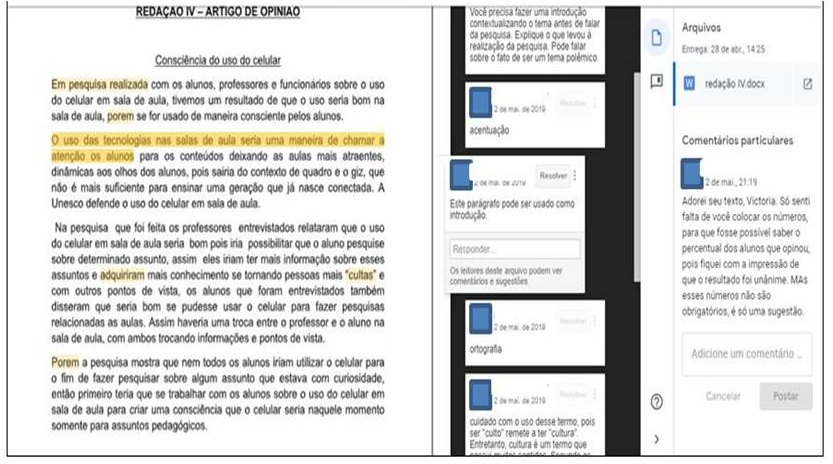
\includegraphics[width=0.8\textwidth]{figure01.png}
    \caption{Acompanhamento da escrita dos alunos}
    \label{fig01}
    \source{Print da tela do computador.}
\end{figure}

Como é possível verificar na \Cref{fig01}, o uso desse recurso foi fundamental para a produção e revisão dos textos, pois propiciou uma maior interação entre os envolvidos no projeto. A mediação da professora foi importante para orientar a escrita dos alunos. Antes de o texto chegar a ser publicado no blog, ele foi revisado pela professora e pelos colegas, num processo de escrita colaborativa. Essa prática se sustenta nas palavras de \textcite{ribeiro2018}, para quem
\begin{quote}
a mesma aula de redação considerando o processo de produção, e não apenas o produto-texto, pode incluir tecnologias que auxiliam o professor no acompanhamento do processo de escrita, seja em tempo real, seja por meio de registros detalhados, para muito além do que era usualmente feito, antes da existência de certos softwares. Do ponto de vista dos alunos, é possível ampliar as condições de interação com colegas, professor, além da pesquisa e da informação que alimentará uma melhor produção de texto \cite[p.~110]{ribeiro2018}.
\end{quote}

Trazer as TDIC para o processo de aprendência faz com que o ensino não fique restrito à sala de aula, pois as interações podem ocorrer a qualquer momento, dependendo da disponibilidade do professor e dos alunos. Além disso, permite um atendimento mais individualizado, aproximando os sujeitos e permitindo que cada qual trabalhe no momento que lhe for mais propício, no seu tempo, ou seja, de forma assíncrona, “aquela em que o aluno realiza as atividades eventualmente recomendadas pelo professor em seu próprio tempo, [bem] como estudar e se preparar para as próximas aulas, ou mesmo realizar avaliações sem contato ao vivo” \cite[p.~12]{almeida2010}.

Após a escrita dos artigos, partimos para a escolha da plataforma que melhor atenderia nosso objetivo de levar o tema escolhido para o rol das discussões sociais. Assim, percebemos que o \emph{blog} reúne características que nos possibilitariam dar continuidade ao nosso trabalho, pois,
\begin{quote}
permite gerar, publicar e trocar conteúdos em formatos múltiplos (vídeo, imagem, áudio) sem a necessidade de contar com uma grande capacitação tecnológica e se relaciona com outros formatos e aplicações na rede, como as páginas web, as redes sociais, os geradores de conteúdos\footnote{Texto original: “(\ldots) permite generar, publicar e intercambiar contenidos en múltiples formatos (vídeo, imagen, audio) sin necesidad de contar con una gran capacitación tecnológica y se relaciona con otros formatos y aplicaciones de la red, como las páginas web, los marcadores sociales, los generadores de contenido \ldots” \cite[p.~8]{fernandez2012}.} \cite[p.~8 - tradução livre nossa]{fernandez2012}.
\end{quote}

Na sequência passamos, então, à criação dos \emph{blogs} que serviriam para a divulgação dos artigos de opinião escritos. Foi realizado, em um primeiro momento, uma aula expositiva, na qual foram apresentados slides que explicavam teoricamente o que é um \emph{blog}. Embora o \emph{blog} seja uma plataforma de acesso fácil e comum aos alunos, eles a utilizam geralmente como fonte de consultas e raramente para a produção textual. Além disso, o fato de trazermos as TDIC para as práticas pedagógicas não significa “um desmonte do que já é praticado, mas cria novas possibilidades de interação, de comunicação, de percepção, de coordenação, enfim, de práticas” \cite[p.~104]{gomes2015}. Desse modo, mesclamos o novo com aquilo que já existia, procurando integrar formas diversas de ensinar e aprender, mostrando que “a presença de tecnologias adaptativas não diminui a importância do professor nas escolas, apenas modifica seu papel” \cite[p.~91]{bacich2015}.

Assim, iniciamos a atividade com uma aula tradicional expositiva, para culminar em um trabalho diferente, em uma aula na qual os alunos assumiram a centralidade do processo, pois tiveram que buscar formas diferentes para criar seus próprios \emph{blogs}. Lembramos que, durante a exposição dos \emph{slides}, acessamos \emph{blogs} diversos e, coletivamente, analisamos as suas estruturas. Percebemos que “a combinação das características de facilidade, ampla divulgação e multimídia tornam o blog uma tecnologia digital com muitas aplicações à prática didática” \cite[p.~98]{gomes2015}.

Após esta aula, os alunos foram até o laboratório de informática para a criação dos seus \emph{blogs}. Neste momento, sugerimos que eles os criassem na plataforma do \emph{Blogger}\footnote{Blogger e Wix são algumas das opções de plataformas para criação de blogs. “Wix é uma plataforma de criação de sites baseada na nuvem, bem simples e grátis para começar. É muito usada por pequenas empresas ou autônomos, que querem um site rápido e de graça. Tem um construtor de sites simples, que não exige praticamente nenhum conhecimento técnico do usuário. [...] O \emph{Blogger} é um serviço gratuito de \emph{blogs} do \emph{Google}. Foi muito popular na virada do milênio e até hoje oferece ótimas funcionalidades, apesar do design não ter acompanhado essa evolução. É bem simples, você precisa apenas de uma conta Gmail para começar” \cite{scotti2021} Disponível em: \url{https://blog.orbitlearn.com/qual-a-melhor-plataforma-para-um-blog-de-sucesso/} Acesso em: 22 abr. 2021.}, do Google, por ser a única que sabíamos manipular. Entretanto, alguns alunos nos surpreenderam dizendo que preferiam criar na plataforma \emph{Wix}, demonstrando seus conhecimentos sobre a questão. Nesse momento, emergiu um processo colaborativo de aprendizagem: os alunos que já conheciam a plataforma orientaram os outros alunos, inclusive a própria professora, mostrando uma horizontalização do processo de aprendência, no qual todos têm algo a aprender e a ensinar ao mesmo tempo. Com esta proposta foi possível desenvolver a percepção de todos os alunos para uma nova prática social na escola, para as novas formas de estudar no século XXI, em que a sociedade é muito mais colaborativa, o que “implica que o estudante precisa ver-se como um agente no mundo, não apenas como um expectador do que nele acontece. Ele precisa ter a consciência de ser um cidadão e de se importar com o que acontece com os seus pares” \cite[p.~104]{gomes2015}.

Durante a criação dos \emph{blogs}, os alunos discutiram questões relacionadas ao \emph{layout}, às imagens que deveriam associar ao texto, à forma como buscariam a participação da sociedade, entre outras.
Como as práticas de transletramento ``envolvem o domínio de habilidades específicas no agenciamento dos múltiplos recursos do ambiente digital''
\cite[p.~188]{sachs2011}, os sujeitos puderam perceber que usar uma única forma de linguagem não lhes permitiria atingir o objetivo proposto.
Considerando os diferentes gêneros
discursivos\footnote{Entendemos gênero discursivo como
  ``[\ldots] um conjunto de convenções relativamente estável que é associado com, e parcialmente representa um tipo de atividade socialmente aprovado, como a conversa informal, comprar produtos em uma loja, uma entrevista de emprego, um Documentário de televisão, um poema ou um artigo científico. Um gênero implica não somente um tipo
  particular de texto, mas também processos particulares de produção, distribuição e consumo de textos'' \cite[p.~161]{fairclough2001}.} que
circulam na sociedade atual, vemos que ``o texto, hoje, é muito mais do que palavra'' \cite[p.~71]{ribeiro2018}, é multissemiótico, e essa
multiplicidade de linguagens converge para a produção de sentidos e, por isso, conforme explica o autor, o ensino da produção textual deve ser pautado na integração de diferentes linguagens, ampliando o poder
semiótico para, assim, alcançar ``a cidadania, a expressão, a compreensão e a capacidade de aprender e de ensinar''.

A multimodalidade é percebida já nas primeiras páginas dos blogs criados pelos alunos, como no exemplo a seguir (\Cref{fig02}):

\begin{figure}[h]
    \centering
    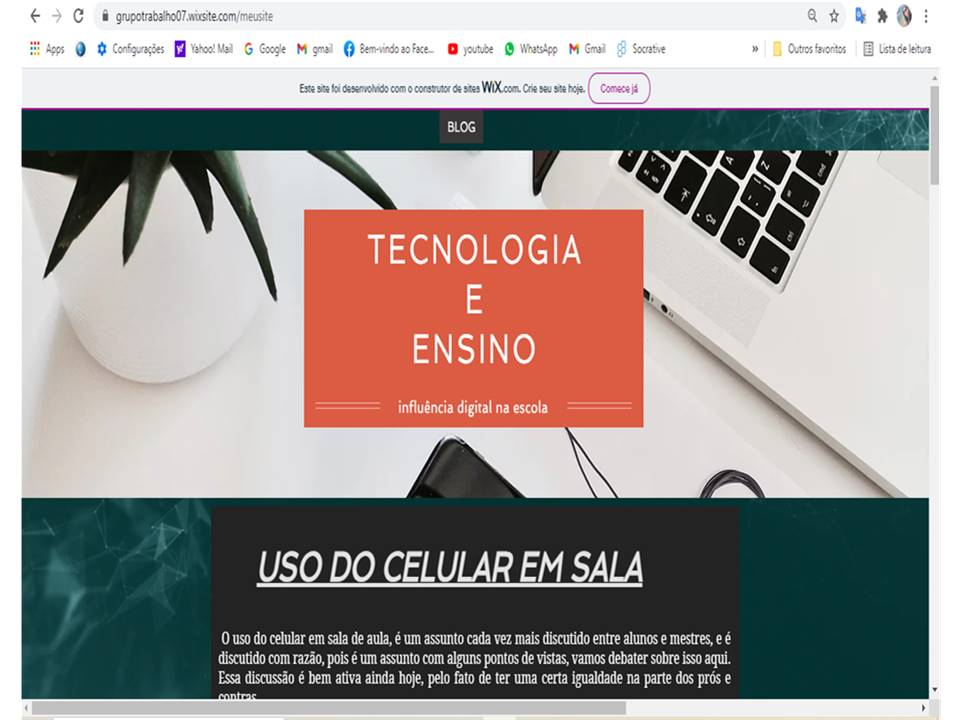
\includegraphics[width=0.8\textwidth]{figure02.png}
    \caption{Página inicial do blog Tecnologia e ensino: influência digital na escola}
    \label{fig02}
    \source{Grupo 7 – Disponível em: \url{https://grupotrabalho07.wixsite.com/meusite}}
\end{figure}

O \emph{blog} como um todo é produzido a partir de uma multissemiose marcante, iniciando com imagens que remetem às tecnologias inovadoras, cores diversas e fortes, bem como a um movimento\footnote{Para visualizar o movimento da tela, acesse o \emph{link} do \emph{blog}.} ao fundo da tela que leva à ideia de futuro. Assim, o desenho da tela principal conduz a essa leitura de algo criativo, buscando atrair o leitor para o tema proposto que aparece já no título “Tecnologia e ensino: a influência digital na escola”, deixando claro o assunto a ser tratado.

Neste contexto, percebe-se que o sentido não está ancorado apenas na linguagem verbal, mas justamente no entrecruzamento dessas formas diferentes de linguagem, ou seja, “a palavra está amalgamada com a imagem, com o som, a cor, o movimento, e aberta à intervenção de quem deseja interagir com ela, com o texto, o discurso, a obra” \cite[p. 57]{dalmolin2003}. Neste processo, a multissemiose é fundamental e não se restringe apenas ao uso de palavras e imagens, mas inclui a escolha das fontes, a forma como os elementos são distribuídos na tela, entre outras. Segundo \textcite{ribeiro2018}:

\begin{quote}
É fundamental, aqui, reposicionar o layout como elemento importante da composição textual, e não apenas como um mero exercício de ‘capricho’ ou ‘ordem’. A distribuição dos textos e de outros modos em uma página de revista, por exemplo, define e é definida por informações, por exemplo, sobre preferências do leitor, partes menos e mais visíveis da página, valores comerciais (por isso mesmo) e saliências de outros tipos \cite[p. 92]{ribeiro2018}.
\end{quote}

Entretanto, é importante ressaltar que o trabalho com o texto multissemiótico não está restrito apenas à sua estrutura visual; inserem-se aí também as relações sociais e culturais nas quais o sujeito está envolvido, uma vez que, ao compor o texto, ele traz consigo toda a sua história, o seu repertório de mundo, seus saberes locais (colocar alguma citação). As escolhas das imagens, dos vídeos, das cores, dos movimentos, ilustram, nessa perspectiva, as relações sociais dos alunos.

Percebemos também que alguns grupos optaram por iniciar a discussão apresentando vídeos sobre o uso do celular em sala de aula e chamando diretamente os leitores para opinarem, participando de uma enquete disponibilizada em um \emph{chat} ou comentando as publicações, conforme podemos verificar no exemplo na \Cref{fig03}.

\begin{figure}[h]
    \centering
    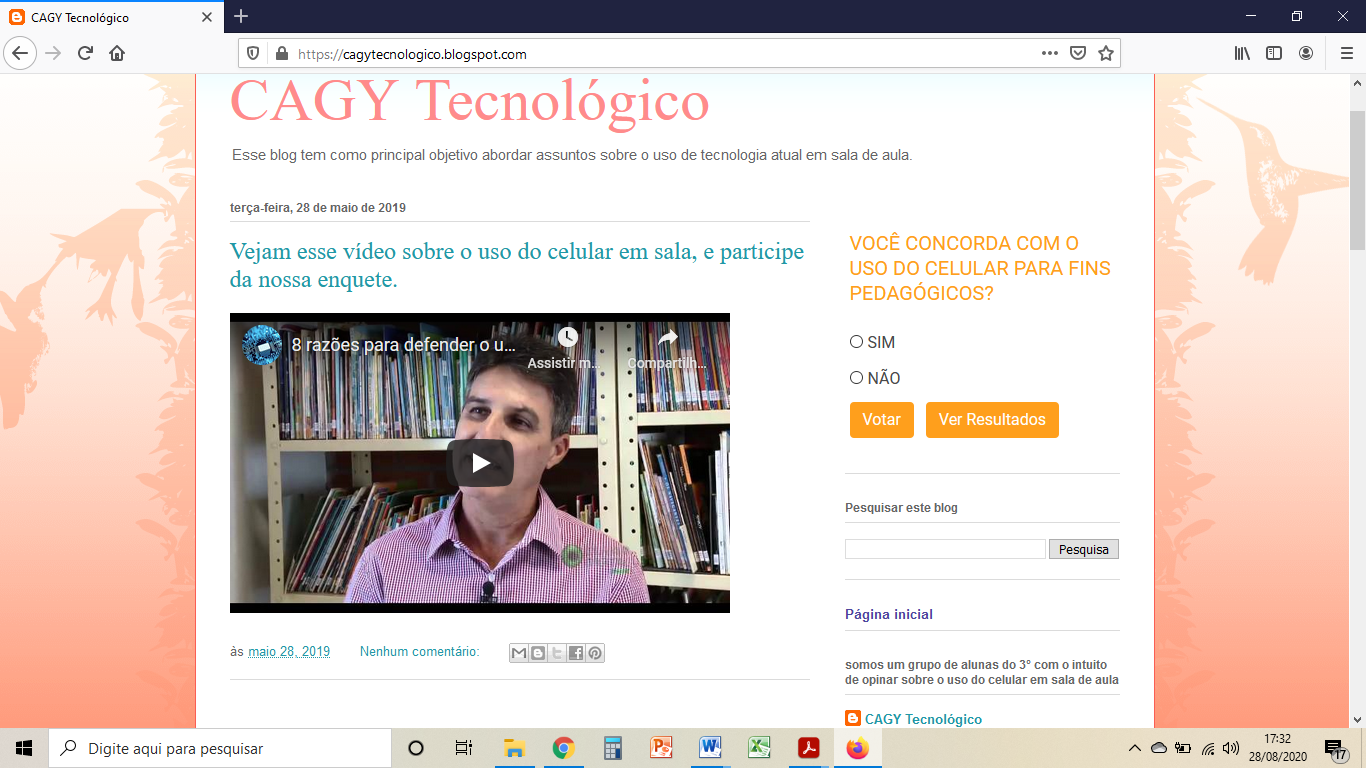
\includegraphics[width=0.8\textwidth]{figure03.png}
    \caption{\emph{Blog}: CAGY tecnológico}
    \label{fig03}
    \source{Disponível em: \url{http://www.cagytecnologico.blogspot.com}}
\end{figure}

O objetivo de levar a problematização do uso do celular para a sala de aula para compor o rol das discussões sociais foi atendido. A afirmação é justificada quando atentamos para os comentários realizados em algumas postagens, conforme é possível ver na \Cref{fig04}.

\begin{figure}[h]
    \centering
    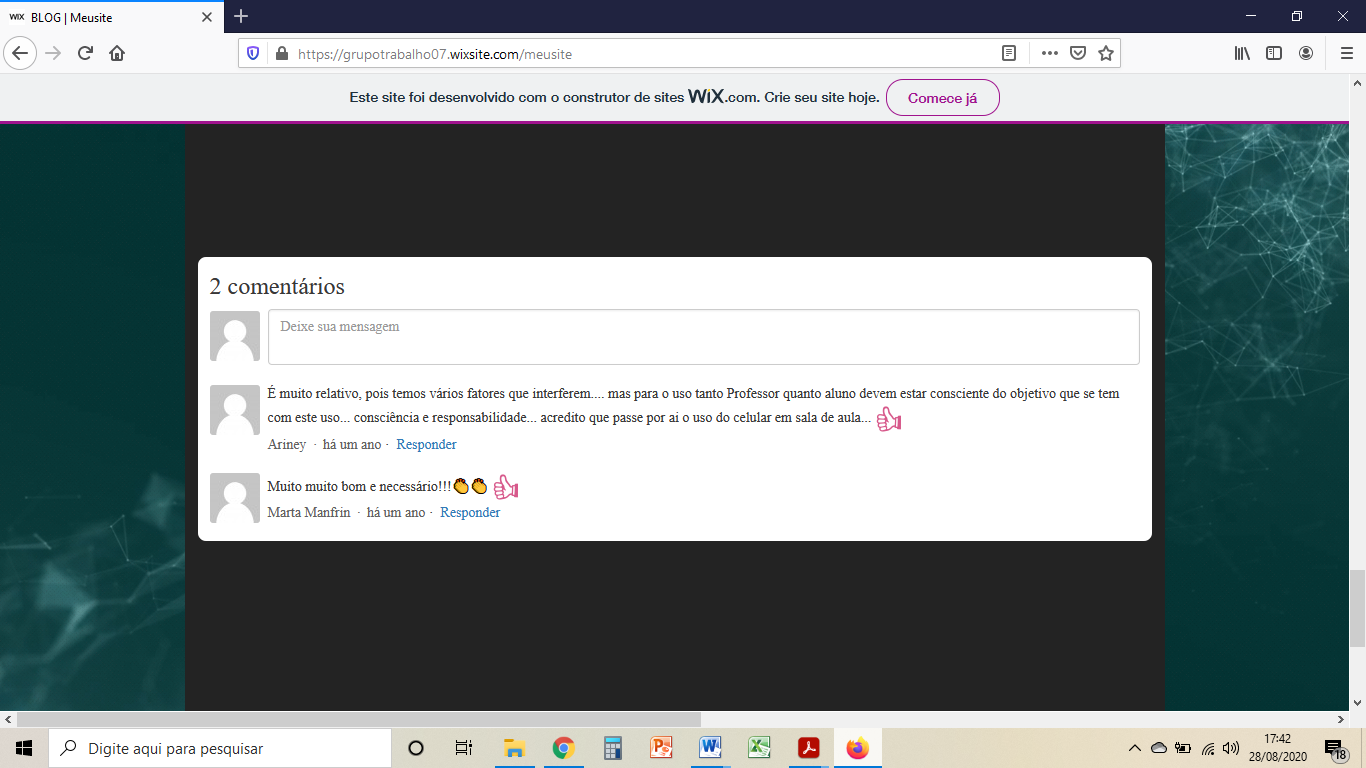
\includegraphics[width=0.8\textwidth]{figure04.png}
    \caption{Comentários feitos no blog Tecnologia e ensino: a influência digital na escola.}
    \label{fig04}
    \source{Grupo 7 – Disponível em: \url{https://grupotrabalho07.wixsite.com/meusite}}
\end{figure}

O que foi estudado na escola extrapolou os limites da sala de aula, estando em conformidade com o que propõe o uso do \emph{blog} como recurso para o processo de aprendência da Língua Portuguesa. Foi possível estabelecer, ademais, o contato com a sociedade como um todo, não mais isolando o aluno na sala de aula. No espaço digital ocorreu a integração de diferentes perspectivas, diferentes modos de ver o mundo, como é possível ver no posicionamento de um dos participantes em relação ao uso do celular em sala de aula para fins de aprendência. Transcrevemos abaixo para facilitar a visualização:

\begin{quote}
É muito relativo, pois temos vários fatores que interferem... mas, para o uso tanto Professor quanto aluno devem estar consciente do objetivo que se tem com este uso... consciência e responsabilidade... acredito que passe por ai o uso do celular em sala de aula.\footnote{O excerto apresentado aqui se refere a um comentário que foi feito por um leitor que acessou o blog criado pelos alunos e deu sua opinião sobre o uso do celular em sala de aula.}
\end{quote}

Observamos que, em seu comentário, o participante deixa claro o seu posicionamento, mostrando que não está nem a favor nem contra o uso do celular em sala de aula. Seu uso depende de se ter “consciência e responsabilidade”, o que vai ao encontro do que os alunos haviam verificado com a pesquisa que realizaram, apresentada por meio de gráficos (\Cref{fig05}).

\begin{figure}[h]
    \centering
    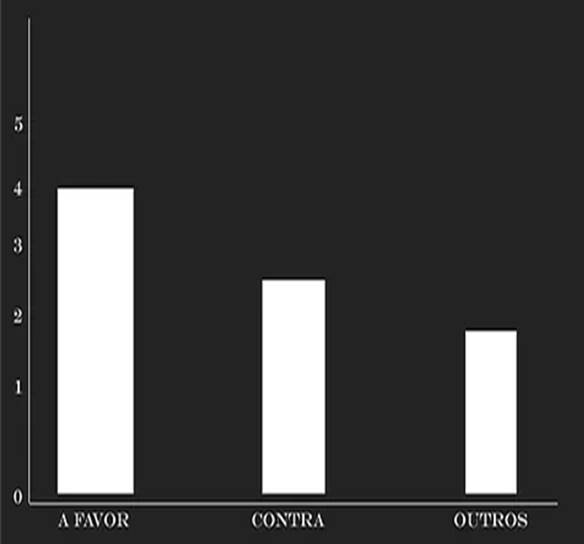
\includegraphics[width=0.5\textwidth]{figure05.png}
    \caption{Gráfico elaborado pelos alunos do grupo 7.}
    \label{fig05}
    \source{\url{https://grupotrabalho07.wixsite.com/meusite}}
\end{figure}

Analisando o gráfico que compõe o artigo de opinião escrito pelos alunos, percebemos que não há um consenso quando o assunto é uso do celular em sala de aula. Tais informações demonstram a importância do tema escolhido, pois ainda temos muito que pesquisar e discutir sobre o uso das TDIC na escola. Além disso, “é preciso que a instituição escolar prepare a população para um funcionamento da sociedade cada vez mais digital e também para buscar no ciberespaço um lugar para se encontrar, de maneira crítica, com diferenças e identidades múltiplas” \cite[p.~7]{rojo2013}.

A atividade de criação dos \emph{blogs} foi apenas uma das práticas de transletramentos das quais os alunos foram protagonistas. Na sequência deste artigo, apresentamos outra proposta de produção, a de foto-haicai. Considerado como sendo um gênero híbrido e multissemiótico, a foto-haicai teve como função sociocomunicativa dar continuidade às reflexões sobre o uso das TDIC nas práticas sociais escolares.



\section{Da fotografia ao haicai e ao foto-haicai: a hibridização na produção de um novo gênero discursivo}\label{sec-fotografia}
\textcite{bakhtin2006} e seu círculo já afirmavam que a linguagem é fundamentalmente dialógica e, segundo \textcite{santaella2012}, nunca esse dialogismo se fez tão presente. A cada novo texto publicado nas redes sociais digitais, inúmeros outros textos vão surgindo; são respostas, comentários etc. Tais textos têm em comum a natureza multissemiótica, posto que, em sua grande maioria, não são constituídos apenas pela linguagem verbal, mas por uma infinidade de outras semioses que ampliam suas possibilidades de sentido. Assim, o ato de ler e escrever, na contemporaneidade, não está restrito à leitura e escrita verbal; leem-se imagens, sons, cores, movimentos.

\begin{quote}
Assim, podemos passar a chamar de leitor não apenas aquele que lê livros, mas também o que lê imagens. Mais do que isso, incluo nesse grupo o leitor da variedade de sinais e signos de que as cidades contemporâneas estão repletas: os sinais de trânsito, as luzes dos semáforos, as placas de orientação, os nomes das ruas, as placas dos estabelecimentos comerciais, etc. Vou ainda mais longe e também chamo de leitor o espectador de cinema, TV e vídeo. Diante disso, não poderia ficar de fora o leitor que viaja pela internet, povoada de imagens, sinais, mapas, rotas, luzes, pistas, palavras e textos \cite[p. 7]{santaella2012}.
\end{quote}

Do mesmo modo, aprendemos a escrever também textos em que a linguagem verbal não detém mais a centralidade, mas divide o espaço com elementos multissemióticos, criando outras possibilidades significativas.

Essa escrita multissemiótica é uma prática bastante comum no cotidiano de grande parte dos adolescentes, posto que estão habituados a produzir textos usando linguagens múltiplas principalmente nas redes sociais, ou seja, tal prática faz parte dos saberes locais desse grupo. Considerando essa realidade, os objetivos propostos e o tema escolhido para as práticas pedagógicas (uso do celular na escola), optamos por trabalhar com os textos fotografia e haicai, de forma conjunta e mesclada, produzindo um novo gênero - a foto-haicai - um gênero híbrido, no qual diferentes estruturas composicionais, estilos e temas misturam-se, dando espaço a outro texto. Segundo \textcite{bakhtin1997}, os gêneros do discurso são relativamente estáveis e esse caráter relativo é o que lhes permite fundir-se com outros gêneros num processo de hibridização. Nas palavras de \textcite[p. 87]{pagano2001}, “nesse processo, os gêneros existentes mudam a partir de modificações na situação social na qual exercem uma função ou novos gêneros podem surgir a partir de transformações ostensivas daqueles já existentes”.

A escolha de inserir a fotografia e o haicai nesta prática social dos alunos se deu pelo fato de ambos capturarem o momento. Isso porque “o trabalho com o haicai e a fotografia possibilita a experiência do conhecimento pelos sentidos, à medida que propõe aos sujeitos a observação atenta, criteriosa de si, do outro, do mundo e das relações que se estabelecem entre esses elementos” \cite[p. 30]{dantas2016}. Assim, a partir da hibridização da fotografia e do haicai, criamos o gênero foto-haicai, por entendermos que ele também captura o momento do pensamento, da visão, do estado de espírito com o uso da linguagem multissemiótica, na qual palavras e imagens se completam.

Para a produção das fotos-haicais, trabalhamos com a técnica denominada “rotação por estações”, ou seja, “os estudantes são organizados em grupos, cada um dos quais realiza uma tarefa, de acordo com os objetivos do professor para a aula em questão” \cite[p. 55]{bacich2015}. Além disso, é importante frisar que, nesta técnica, os estudantes podem realizar atividades coletivas, de forma colaborativa ou individualmente.

Na atividade realizada por meio da rotação de estações, os alunos foram organizados em grupos de até 05 (cinco) participantes e cada grupo pesquisou sobre um tema específico, usando seu celular ou o notebook que foi levado à sala de aula. Os temas estavam relacionados aos gêneros discursivos fotografia e haicai. A cada 10 minutos, os alunos mudavam de estação, pesquisando outro aspecto relacionado aos gêneros em foco. Ao final das pesquisas, fizemos um debate para compartilhar as descobertas. Neste tipo de atividade, o professor passa a ser mediador do processo, não trazendo para si a centralidade das atividades. O seu papel passa a ser o de:

\begin{quote}
Ditar o ritmo, a dinâmica que o atende melhor e entender que cada atividade tem um objetivo a ser alcançado. O professor passa a ser um coadjuvante, um facilitador para que os estudantes alcancem o objetivo. Assim, a ação do professor passa a ser pontual e, como facilitador, ele atua se necessário. Quando o aluno tem alguma dificuldade, o professor não apresenta a solução para o problema, mas indica o caminho a percorrer para que o próprio aluno busque solução. Assim, o professor garante indivíduos bem-sucedidos nas aulas e na vida \cite[p. 84]{pires2015}.
\end{quote}

Atuando na condição de mediador, o professor incentiva seus alunos a buscarem informações sobre os gêneros discursivos propostos. Inclusive, a escolha do gênero partiu de uma solicitação dos próprios alunos, pois foram eles que pediram para estudarmos os haicais e decidimos, coletivamente, unir o haicai e a fotografia. Então, com a atividade proposta, foi possível conhecer as características dos gêneros fotografia e haicai e, na sequência, passar a produzi-los. Para tal, utilizando seus \emph{smartphones}, os alunos espalharam-se pela escola e produziram fotos nas quais as imagens estavam relacionadas ao uso dos recursos tecnológicos e das tecnologias digitais na escola. Estas fotos poderiam ser de algo que estivesse pronto ou de algo que eles montassem, usando objetos diversos. Na sequência, acrescentaram o texto verbal, em formato de haicais, às fotos produzidas surgindo, assim, as fotos-haicais. A seguir, podemos ver (\Cref{fig06}) um exemplo do trabalho realizado:

\begin{figure}[h]
    \centering
    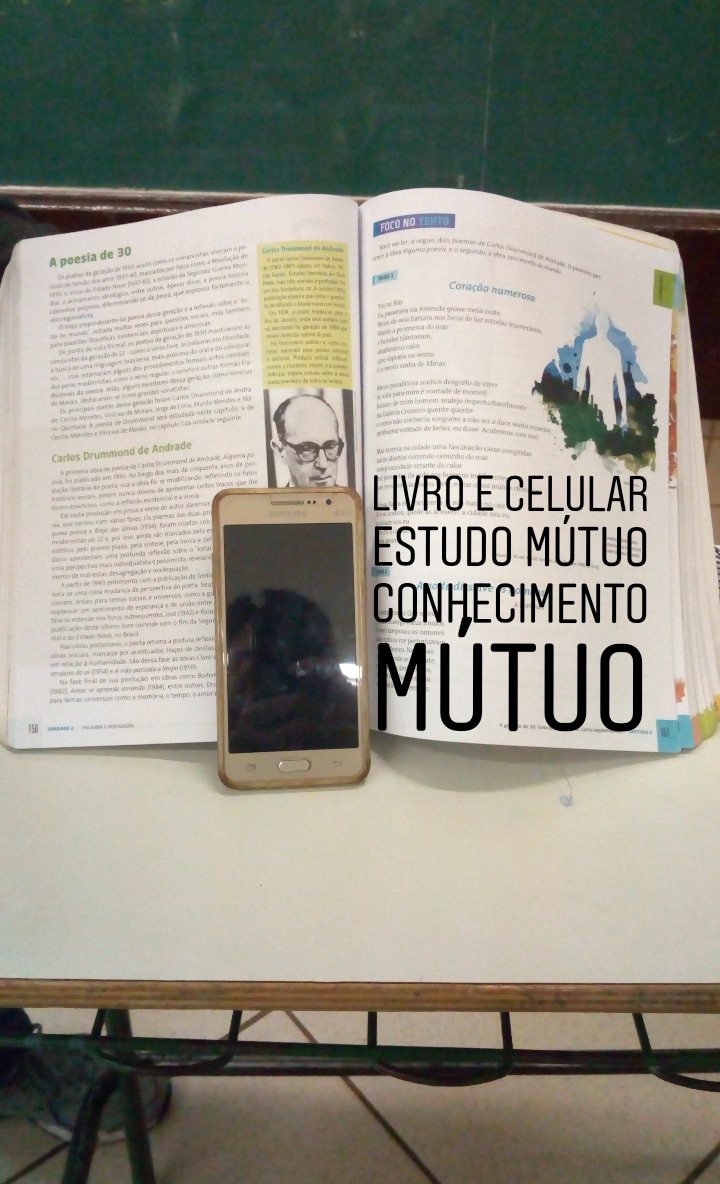
\includegraphics[width=0.5\textwidth]{figure06.png}
    \caption{Foto-haicai produzida pelo aluno José.}
    \label{fig06}
    \source{arquivo da professora}
\end{figure}

A forma como os objetos foram dispostos para a produção da fotografia associada à linguagem verbal produz um possível sentido pretendido por seu autor. Os elementos não verbais são atravessados pelos elementos verbais e a junção de todos eles constitui o texto como um conjunto. Percebe-se que “a imagem é claramente topológica, ou seja, ocupa espaços, enquanto a linguagem oral e escrita é tipológica e distribui-se no tempo” \cite[p. 22]{rojomoura2019}. Aliás, toda a produção remete à ideia de hibridismo entre as formas tradicionais de aprendizado representadas pelo livro e as TDIC que são representadas pelo celular e corroborada pelo uso da palavra “mútuo”, indicando que as duas formas, juntas, contribuem para o aprendizado.

\textcite{barbosa2015} afirmam que no gênero híbrido não há fronteiras; a fusão em um único enunciado é completa. Embora o gênero foto-haicai mantenha características da fotografia e do haicai, elas não estão mais separadas, são agora características que pertencem a este novo gênero discursivo que surgiu da hibridização. A imagem que captura o instante da visão, característica da fotografia, agora é parte fundamental da foto-haicai, na qual se agregam as palavras. Sendo assim, imagens e palavras são características fundamentais para a construção dos sentidos nesse gênero textual, conforme pode ser verificado no próximo exemplo (\Cref{fig07}):

\begin{figure}[h]
    \centering
    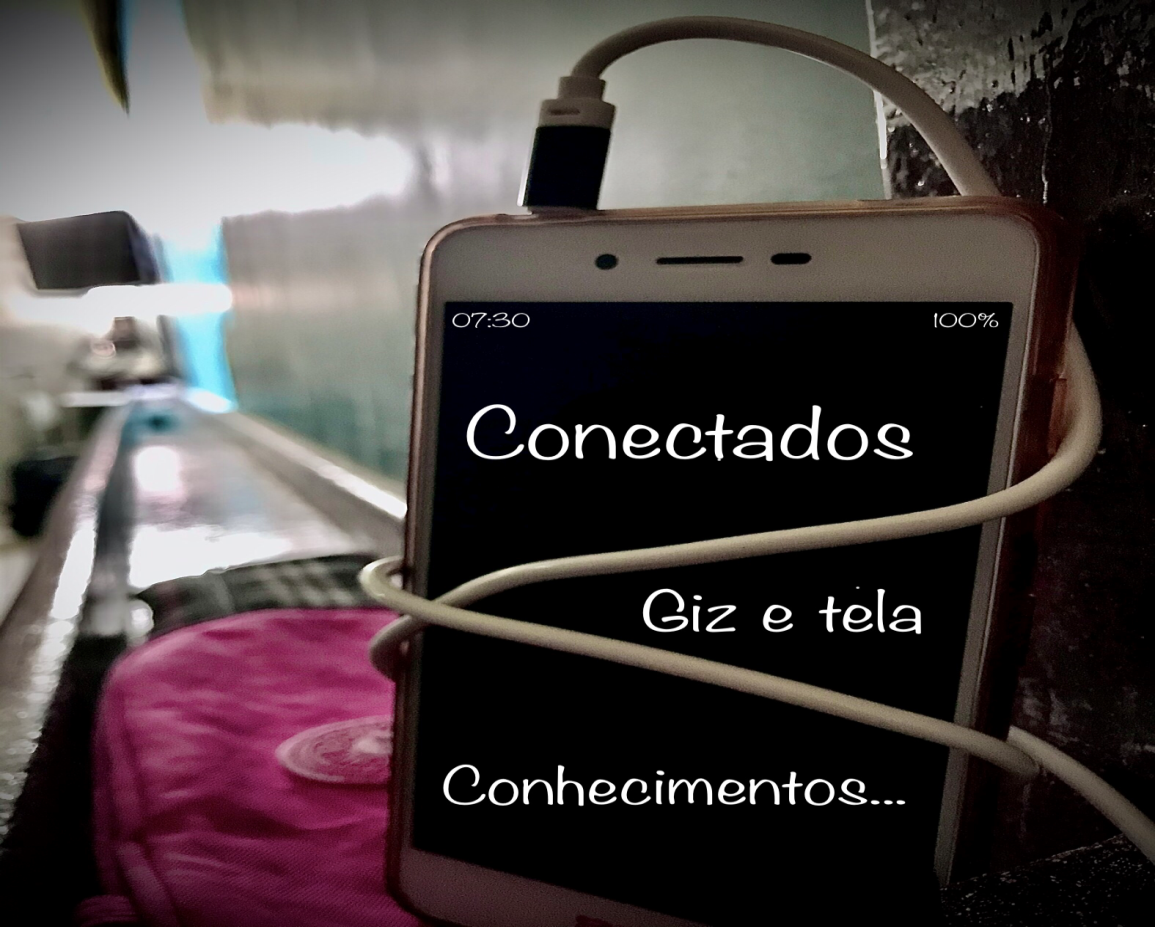
\includegraphics[width=0.7\textwidth]{figure07.png}
    \caption{Foto-haicai produzida pela aluna Ana.}
    \label{fig07}
    \source{arquivo da professora}
\end{figure}

Percebemos essa noção de hibridização em todos os aspectos do texto. Vemos que ele mantém as características desse novo gênero, a foto-haicai, uma vez que a linguagem verbal e a não verbal estão entrelaçadas e não há forma de separá-las para que os sentidos sejam produzidos. A imagem nos mostra um celular sobre um estojo escolar encostado em um quadro-negro, revelando que essas tecnologias digitais já estão na sala de aula, fazendo parte dela. Essa ideia de que a aula está interligada com as TDIC é corroborada pela linguagem verbal que sugere a conexão do giz com a tela e os conhecimentos, reforçada pela imagem do cabo envolvendo o celular, mostrando que estão todos entrançados.

Este entrelaçamento presente na foto-haicai da aluna Ana (\Cref{fig07}), transparece elementos de suas práticas escolares, seu modo de agir no mundo, pois “o conhecimento é sempre tradução e reconstrução do mundo exterior e permite um ponto de vista crítico sobre o próprio conhecimento” \cite[p. 53]{morin_saberes_2010}. O conhecimento da aluna sobre a sua realidade é ressignificado e evidencia seus “saberes locais”, deixando claro que estes jamais desaparecerão \cite{geertz1997}.

\section{Considerações finais}\label{sec-consideracoes}
O objetivo desse artigo foi discutir como práticas pedagógicas ancoradas nos transletramentos podem contribuir, reciprocamente, para a formação crítica ampliada do professor e dos alunos, nas aulas de Língua Portuguesa da 3ª série do Ensino Médio de um Colégio Estadual, na região da Tríplice Fronteira Brasil/Paraguai/Argentina.

Considerando a formação crítica ampliada da professora e dos alunos, todos foram envolvidos em práticas de transletramentos, nas quais seus saberes locais puderam ser explicitados, tendo as TDIC como recursos fundamentais do processo de aprendência. Além disso, a proposta ainda mostrou que é possível desenvolver a participação ativa do aluno, tornando-o corresponsável e protagonista do seu aprendizado e desenvolvimento, tirando a centralidade do professor.

Argumentamos, então, que é função de toda comunidade escolar a revisão permanente das práticas pedagógicas, posto que, como integrante da sociedade do século XXI, precisamos acompanhar esta revolução digital pela qual estamos passando. Não se trata de trazer as TDIC para o contexto escolar, visto que elas já estão presentes nas diferentes práticas sociais dos alunos e professores; trata-se de convertê-las em práticas que possam auxiliar no processo de aprendência, ou seja, no processo de formação desse sujeito contemporâneo.

Em se tratando especificamente da disciplina de Língua Portuguesa, que se constitui pelo trabalho com os diferentes gêneros discursivos, a necessidade de trazer as TDIC para a sala de aula é ainda mais emergente, uma vez que as interações sociais ocorrem, em sua grande maioria, através de textos digitais que são, em sua essência, multissemióticos. Nos textos produzidos pelos alunos, os sentidos são produzidos em um processo intermidiático, onde é impossível separar as múltiplas semioses que os constituem.

Assim, a proposta de ensino apresentada compreende a prática de ensino da Língua Portuguesa como uma forma de interação entre sujeitos de contextos diversos, indo além dos muros da escola. A proposta possibilitou aos alunos ampliarem os sentidos do texto, não o tomando como uma simples abstração, uma simples tarefa a ser cumprida, mas como uma prática social que faz parte de seu cotidiano. Dessa forma, o ensino se torna muito mais significativo, visto que ao serem trazidas para a sala de aula recursos que fazem parte das diferentes práticas sociais dos alunos, recursos com as quais já estavam familiarizados, os seus saberes locais são valorizados, tornando as aulas mais atrativas e contribuindo para que sejam sujeitos ativos desse processo.

Atualizar a escola e os processos de aprendência não significa trazer grandes inovações, mas seguir o rumo em que se encontra a sociedade do século XXI, em razão de que não há como retroceder. Permanecer preso ao passado é manter a escola longe da atual realidade, como se houvesse uma forma de comunicação fora do espaço escolar e outra, dentro dele.



\printbibliography\label{sec-bib}
% if the text is not in Portuguese, it might be necessary to use the code below instead to print the correct ABNT abbreviations [s.n.], [s.l.] 
%\begin{portuguese}
%\printbibliography[title={Bibliography}]
%\end{portuguese}

%full list: conceptualization,datacuration,formalanalysis,funding,investigation,methodology,projadm,resources,software,supervision,validation,visualization,writing,review
\begin{contributors}[sec-contributors]
\authorcontribution{Adriane Elisa Glasser}[conceptualization,datacuration,investigation,projadm,supervision,validation,visualization,writing,review]
\authorcontribution{Maria Elena Pires Santos}[conceptualization,projadm,supervision,validation,visualization,writing,review]
\end{contributors}


\end{document}
